\documentclass[border=0mm]{standalone}
\usepackage{fontspec}
\usepackage{unicode-math}
\usepackage{tikz}
\usetikzlibrary{arrows.meta, positioning}
\setmainfont{Linux Libertine O}
\setsansfont{Linux Biolinum O}

\begin{document}
	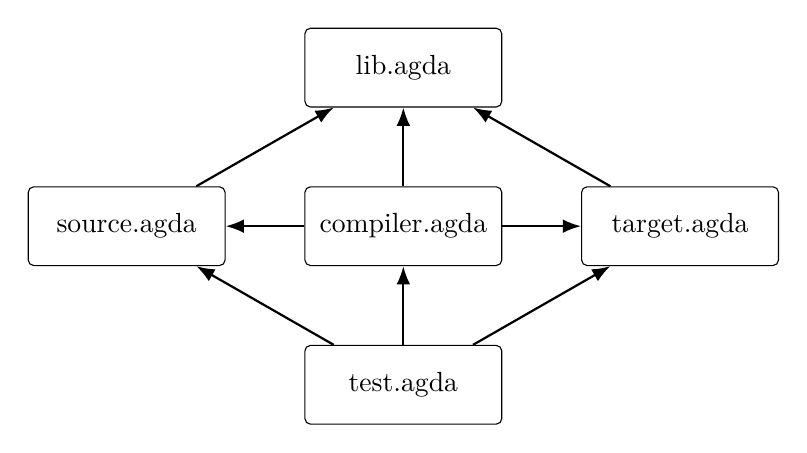
\begin{tikzpicture}[
		node distance=1cm and 1cm,
		every node/.style={draw, rounded corners=2pt, minimum width=2.5cm, minimum height=1cm, align=center},
		arrow/.style={-{Latex}, thick}
	]
	
		% Nodes
		\node (lib) {lib.agda};
		\node[below left=of lib] (source) {source.agda};
		\node[below right=of lib] (target) {target.agda};
		\node[below =of lib] (compiler) {compiler.agda};
		\node[below =of compiler] (test) {test.agda};
		
		% Arrows
		\draw[arrow] (source) -- (lib);
		\draw[arrow] (target) -- (lib);
		\draw[arrow] (compiler) -- (source);
		\draw[arrow] (compiler) -- (target);
		\draw[arrow] (compiler) -- (lib);
		\draw[arrow] (test) -- (source);
		\draw[arrow] (test) -- (target);
		\draw[arrow] (test) -- (compiler);

		
	\end{tikzpicture}
\end{document}
